\chapter{Related work}
\label{chp:related-work}

The field of energy harvesting devices is promising, but still immature and only a few companies provide such devices commercially. We give an overview of several energy harvesting platforms, both research related and commercial.

Writing software for intermittent devices comes with the challenge of handling frequent and random power cycles. We will discuss which programming models have been developed to counter this issue.

For batteryless, intermittently powered devices there are no publicly available testbeds. Work of \cite{request} enlists properties and features that such a testbed should have, as well as presenting a minimal implementation. The authors call for a more coordinated action in this domain research.

On the other hand there are dozens of existing testbeds for battery-based wireless sensor networks (WSN). There have been many survey published in the past years that compare each of them in detail (see for instance \cite{survey1}, \cite{survey2}). Our goal here is to revise these comparative studies expanding it with the recent developments in testbed deployments.

Besides these testbeds, we will discuss several tools which help in developing applications for batteryless devices.

\section{Energy harvesting platforms}

In this section a brief overview is given of batteryless energy harvesting platforms using various energy sources. This has been surveyed in \cite{sudevalayam2011energy}, \cite{energywsn} ,\cite{talla2015powering} and \cite{kim2014ambient}. Energy harvesting and it's potential with respect to WSNs has been surveyed in \cite{akhtar2015energy} and \cite{bhatti2016energy}.

Table \ref{tab:researchplatforms} shows some popular and recent developed platforms in scientific research. In Table \ref{tab:commercialplatforms} show several companies which are commercially active in the field of energy harvesting devices.

{\renewcommand{\arraystretch}{1.5}
\begin{table*}\footnotesize
\makebox[\linewidth]{ \begin{tabularx}{1.5\textwidth}{sXssssts}
	\toprule
	\textbf{Platform} & \textbf{Description} & \textbf{MCU} & \textbf{Radio} & \textbf{Energy Harvester} & \textbf{Energy Source} & \textbf{Year} & \textbf{Citations}\\
	\midrule

	WISP \cite{wisp} & Family of sensors that are powered and read by UHF RFID readers & MSP430 & \hspace{0pt}Backscattering & Transducer and rectifiers & RF & 2008 & 639 \\
	
	Flexible AD PZT Energy Harvester \cite{aerol} & Self-Powered Wireless Sensor Node Enabled by an Aerosol-Deposited PZT Flexible Energy Harvester & MSP430 & CS2500 & Flexible piezoelectric energy harvester & Kinetic & 2016 & 65\\
	
	Umich Moo \cite{moo} & Improvement on design of WISP & MSP430 & \hspace{0pt}Backscattering & Transducer and rectifiers & RF & 2011 & 63 \\

	Monjolo \cite{monjolo} & Energy-Harvesting AC Power metering which draws zero power under zero load conditions & MSP430 & CC2420 & CR2550, LTC3588 & Power line energy harvesting (magnetic field) & 2013 & 45\\
	
	SPWTS \cite{spwts} & A novel self-powered wireless temperature sensor based on thermoelectric generators & nRF24LE1 & Build in MCU & TEC12706 & Thermal & 2014 & 31\\
	
	Flicker \cite{flicker} & Configurable development board for batteryless IoT & MSP430 & CC1101, nRF51822, backscattering & Solar cell, transducer and rectifiers, LTC3588,  & Solar, RF, Kinetic & 2017 & 11 \\
	
	Capybara \cite{capybara} & Co-designed hardware/software power system with dynamically reconfigurable energy storage capacity & MSP430, CC2650 & CC2650 & TrisolX solar panels, low-power voltage source & Solar, energy source emulation & 2018 & 11 \\
	
	Pible \cite{pible} & BLE batterlyless platform & CC2650 & Build in MCU & Solar panels & Solar & 2018 & 2 \\	
	
	\bottomrule
\end{tabularx}}
\caption{Research Based Energy Harvesting Platforms.}
\label{tab:researchplatforms}
\end{table*}}

{\renewcommand{\arraystretch}{1.5}
\begin{table*}\footnotesize
\makebox[\linewidth]{ \begin{tabularx}{1.5\textwidth}{sXssss}
	
	\toprule
	\textbf{Company} & \textbf{Description} & \textbf{MCU} & \textbf{Radio} & \textbf{Energy Harvester} & \textbf{Energy Source}\\
	\midrule
	
	EnOcean & Various batteryless solutions for i.e.Building Automation and Smart Home & 8051 processor & TCM 3x0 & ECO 200, ECS 300, ECT 310 Perpetuum & Solar, motion, thermal\\

	Powercast & Provides wireless power solutions, RFID tags, RF power transmitter,  RF power harvester & PIC24F & IEEE 802.15.4 transceiver, TX91502 & PCC110 & RF\\
	
	Williot & Makes a batteryless bluetooth beacon device based on RF harvesting & ARM processor & N/A & N/A & RF\\
	
	PsiKick & Provides batteryless monitoring solutions to mainly the industry. Related to the university of Virginia and Michigan. & Custom ULP SoC, ARM architecture \cite{customsoc} & Build in SoC & N/A & Solar, thermal\\
	
	Bellutech & BelluTech’s patented batteryless wireless miniature sensors continuously track and record exposure to environmental and operating conditions. & N/A & N/A & N/A & RF\\	
	
	Matrix Industries & Makes a batteryless thermoelectric powered smartwatch & N/A & N/A & N/A & Thermal\\

	\bottomrule
\end{tabularx}}
\caption{Commercial Energy Harvesting Platforms.}
\label{tab:commercialplatforms}
\end{table*}}


\section{Programming Models For Intermittent Computing}
\begin{figure}[htb]
	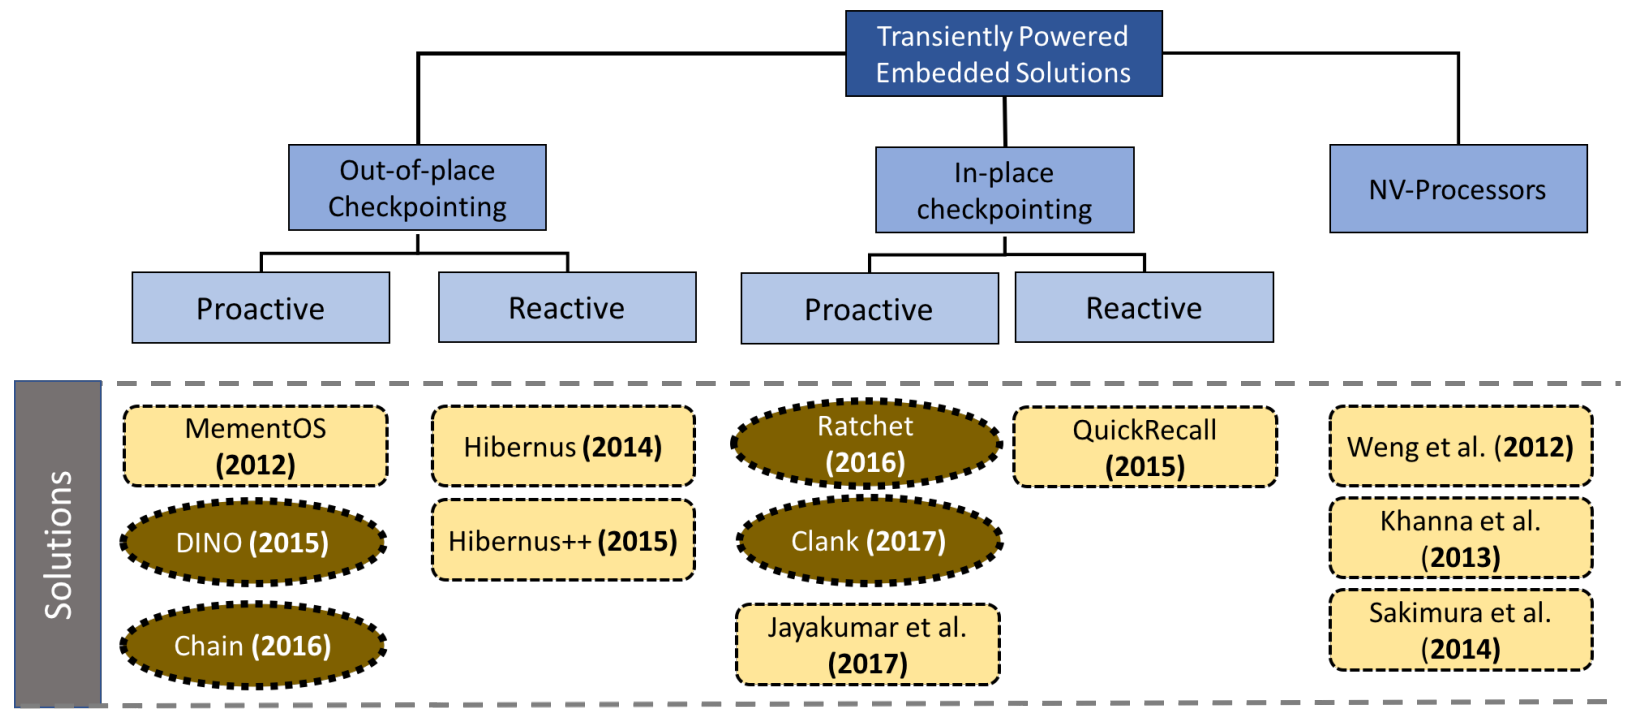
\includegraphics[width=\textwidth]{pics/taxonomy-tpc}
	\caption{Taxonomy of several programming models for intermittent computing \cite{tpcthesis}.}
	\label{fig:architecture}
\end{figure}


\section{Wireless Sensor Network Testbeds}
\label{sec:wireless-sensor-networks}
\todo{Paraphrase this section, taken from https://www.iotbench.ethz.ch/}

\subsection{FIT IoT-LAB}
FIT IoT-LAB \cite{FIT-IoT} provides a very large scale infrastructure facility suitable for testing small wireless sensor devices and heterogeneous communicating objects.

IoT-LAB features over 2000 wireless sensor nodes spread across six different sites in France.  Nodes are either fixed or mobile and can be allocated in various topologies throughout all sites.  A variety of wireless sensors are available, with different processor architectures (MSP430, STM32 and Cortex-A8) and different wireless chips (802.15.4 PHY @ 800 MHz or 2.4 GHz).  In addition, “open nodes” can receive custom wireless sensors for inclusion in IoT-LAB testbed.

\subsection{Flocklab}

Flocklab \cite{flocklab} is a wireless sensor network (WSN) testbed, developed and run by the ​Computer Engineering and Networks Laboratory at the ​Swiss Federal Institute of Technology Zurich (ETH Zurich) in Switzerland. FlockLab's key features include:
\begin{itemize}
	\item FlockLab's observer based testbed architecture which provides services for detailed testing of sensor nodes:
	\item Time accurate pin tracing
	\item Time accurate pin actuation
	\item Power measurements
	\item Serial interface logging and writing
	\item Voltage control to simulate e.g. battery depletion
\end{itemize}

\subsection{Indriya2}

Indriya2 \cite{indriya2} is a three-dimensional wireless sensor network deployed across three floors of the School of Computing , at the National University of Singapore (NUS). The Testbed facilitates research in sensor network programming environments, communication protocols, system design, and applications. It provides a public, permanent framework for development and testing of sensor network protocols and applications. Users can interact with the Testbed through an intuitive web-based interface designed based on Harvard's Motelab's interface. Registered users can upload executables, associate those executables with motes to create a job, and schedule the job to be run on Testbed. During the job execution, all messages and other data are logged to a database which is presented to the user upon job completion and then can be used for processing and visualization. 

\section{Development Tools For Batteryless Devices}

\todo{Make this section more technical, provide a table comparing tools and add introductory paragraph}

\subsection{Ekho}

To counter the issue of randomness in a energy harvesting power source, Ekho \cite{ekho} has been developed. This an emulator capable of accurately recreating harvesting conditions in a lab. It reproduces the I-V characteristics of energy harvesting sources, allowing developers to choose from a library of energy traces recorded with various sources and environmental conditions.

\subsection{Flicker}
\todo{Paraphrase this section}
Flicker \cite{flicker} is a platform for quickly prototyping batteryless embedded sensors. Flicker is an extensible, modular, “plug and play” architecture that supports RFID, solar, and kinetic energy harvesting; passive and active wireless communication; and a wide range of sensors through common peripheral and harvester interconnects. Flicker supports recent advances in failure-tolerant timekeeping, testing, and debugging, while providing dynamic federated energy storage where peripheral priorities and user tasks can be adjusted without hardware changes.

\subsection{Energy aware debugger}
\todo{Paraphrase this section}
The Energy-Interference-Free Debugger (EDB) \cite{edb}, is a tool for monitoring and debugging of intermittent systems without adversely affecting their energy state. EDB recreates a familiar debugging environment for intermittent software and augments it with debugging primitives for effective diagnosis of intermittence bugs.



